\begin{definition}
    Алгебра Гейтинга (псевдобулева алгебра)~--- импликативная решетка с 0.
\end{definition}

\begin{definition}
    Введем операцию $\sim a \equiv a \to 0$~--- дополнение до 0.
\end{definition}
\begin{definition}
    Булева алгебра~--- Алгебра Гейтинга, где $a + \sim a = 1$.
\end{definition}

\begin{example}
    Булева Алгебра

    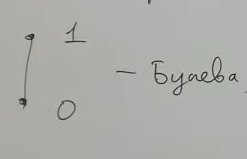
\includegraphics[scale=0.8]{img/bool_algebra}

    \begin{itemize}
        \item $\cdot$ соответствует $\&$,
        \item $+$ соответствует $\vee$,
        \item $\to$ соответствует $\to$,
        \item $\sim$ соответствует $\neg$.
    \end{itemize}
\end{example}

Далее $\alpha, \beta$~--- высказывания в ИИВ.

\begin{definition}
    $\alpha \leqslant \beta$, если $\alpha \vdash \beta$
\end{definition}

\begin{definition}[Равносильность высказываний]
    $\alpha \approx \beta$, если $\alpha \leqslant \beta$ и $\beta \leqslant \alpha$
\end{definition}

\begin{definition}[Алгебра Линденбаума]
    Пусть $\xi$~--- множество всех высказываний ИИВ.

    $[ \xi ]$ (множество классов эквивалентности высказываний по отношению $\approx$) называется алгеброй Линденбаума $\mathcal{L}$.
\end{definition}

\begin{theorem}
    $\mathcal{L}$ (алгебра Линденбаума) --- Алгебра Гейтинга.
\end{theorem}

Введем оценку высказывания в алгебре Линденбаума. Отобразим $\llbracket\alpha\rrbracket = [\alpha]$ (то есть оценка $\alpha$ есть ее класс эквивалентности).

\begin{lemma}
    $\mathds{1} = [A \to A]$
\end{lemma}

\begin{proof}
    $\alpha \vdash A \to A$, верно (очевидно), то есть $[\alpha] \leqslant [A \to A]$, то есть $[A \to A] = \mathds{1}$.
\end{proof}

\begin{theorem}
    $\mathcal{L}$~--- корректная модель ИИВ.
\end{theorem}

\begin{proof}
    Действительно, каждая формула имеет оценку, оценки представляются в виде решетки по отношению доказуемости. Если $[\alpha] = [A \to A]$, то и $\llbracket \alpha \rrbracket = [A \to A]= \mathds{1}$.
\end{proof}

\begin{theorem}
    $\mathcal{L}$~--- полная модель ИИВ.

\end{theorem}

\begin{proof}
    $\vDash \alpha$, то есть $[\alpha] = \mathds{1}$.

    $\llbracket\alpha\rrbracket = \mathds{1}$, значит $\llbracket\alpha\rrbracket = [A \to A]$, это есть что $\alpha$ эффективна $\mathds{1}$, то есть $\beta \leqslant [\alpha]$ при всех $\beta$.

    Возьмем $\beta = A \to A$. Докажем, что $\vdash \alpha$.
    \begin{itemize}
        \item[1-5)] $A \to A$
        \item[6)] $A \to A \to \alpha$ (теорема о дедукции)
        \item[7)] $\alpha$
    \end{itemize}
\end{proof}

\begin{theorem}
    Алгебра Гейтинга (все возможные ее модели)~--- полная и корректная модель ИИВ.
\end{theorem}

\begin{proof}
    \textbf{Полнота.} Если формула $\alpha$ истинна в любой алгебре Гейтинга, значит она истинна и в алгебра Линденбаума, а она является полной моделью ИИВ.
\end{proof}

\begin{definition}
    Исчисление дизъюнктно, если для любых $\alpha, \beta\quad \vdash \alpha \lor \beta$ влечёт $\vdash \alpha$ или $\vdash \beta$.
\end{definition}

\begin{theorem}
    ИИВ дизъюнктно.
\end{theorem}

\begin{definition}
    Пусть существует $f: A \to B, \quad A, B$ -- алгебры Гейтинга.

    $f$ -- гомоморфизм, если $f(0_A) = 0_B\quad f(1_A) = 1_B$ и $f(\alpha \star_A \beta) = f(\alpha) \star_B f(\beta)$
\end{definition}

\begin{definition}[Геделева Алгебра]
    Это такая алгебра, где $a + b = 1$ влечет $a = 1$ или $b = 1$.
\end{definition}

\begin{definition}
    [$\Gamma (A)$]
    Пусть $A$~--- алгебра Гейтинга.

    Определим $\gamma: A \to \Gamma(A)$ так:
    $\gamma(x) = \begin{cases}
        \omega, &x = 1_A\\
        x, & x < 1_A\\
    \end{cases}$
    и добавим $1_{\Gamma(A)}$: $t \leqslant 1_\Gamma(A)$, если $t \in \Gamma(A)$.

    \begin{center}
        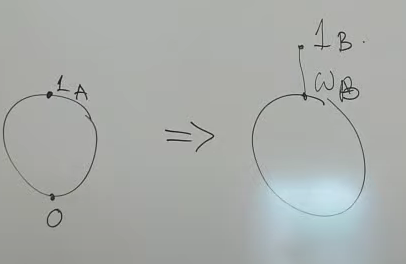
\includegraphics[scale=0.5]{img/gedelerisation.png}
    \end{center}
\end{definition}

\begin{remark}
    $\Gamma (A)$ неофициально называется Геделеризацией.
\end{remark}

\begin{theorem}
  $\Gamma(A)$ -- Гёделева алгебра.
\end{theorem}
\begin{proof}
    Пусть $a+b = 1_{\Gamma(A)}$, посмотрим на картинку.
\end{proof}

\begin{definition}
    Каноническое отображение $g(x): \Gamma(\mathcal L) \to \mathcal L$\\
    $g(x) = \begin{cases}
        1,& x = 1 \text{ или } \omega\\
        x,& \text{ иначе}\\
    \end{cases} $.
\end{definition}
\begin{statement}
        $g(x)$ -- гомоморфизм
\end{statement}

\begin{statement}
    $\Gamma(\mathcal L)$~--- Гёделева алгебра.
\end{statement}

\begin{theorem}
    Рассмотрим ИИВ и алгебры Гейтинга $\mathcal L, \Gamma (\mathcal{L})$
\end{theorem}

\begin{statement}
    Если $g: A \to B$ и $\llbracket\alpha\rrbracket_A = 1_A$, то
    $\llbracket \alpha \rrbracket_B = g(1_A)$.
\end{statement}


\begin{proof}[Доказательство теоремы о дизъюнктности ИИВ]

    Рассмотрим $\vdash \alpha \vee \beta$.

    $\Gamma (\mathcal L)$~--- Гёделева алгебра, то есть алгебра Гейтинга.

    $\llbracket \alpha \lor \beta \rrbracket_{\Gamma(\mathcal L)} = 1_{\Gamma(\mathcal L)}$,
    т.е. либо $\llbracket \alpha \rrbracket =1_{\Gamma({\mathcal L})}$, либо $\llbracket \beta \rrbracket _{\Gamma(\mathcal L)} = 1_{\Gamma(\mathcal L)}$.

    Рассмотрим $g : \Gamma(\mathcal{L}) \to \mathcal{L}$

    $\llbracket \alpha \rrbracket _{\Gamma(\mathcal L )} = 1_{\Gamma(\mathcal L)}$, тогда $\llbracket \alpha \rrbracket _{\mathcal L} = g(1_{\Gamma(\mathcal L)}) = 1_{\mathcal L}$

    т.е. $\vdash \alpha$.
\end{proof}

\begin{definition}
    Модель ИИВ называется табличной, если\begin{itemize}
        \item $\mathbb{V} = \mathcal S$~--- множество истинностных значений;
        \item $\llbracket \alpha \star \beta \rrbracket = f_\star \left( \llbracket \alpha \rrbracket, \llbracket \alpha, \beta \rrbracket \right)$,
        \item  Существует $\true \in \mathcal{S}$ -- выделенная истина $\llbracket \alpha \rrbracket = \true$ тогда и только тогда, когда $\vDash \alpha$.
    \end{itemize}

\end{definition}

\begin{definition}
    Конечная табличная модель~--- модель, где $\mathbb V$~--- конечная.
\end{definition}

\begin{note}
    Оценка работает так:
    $\llbracket P_i \rrbracket = f_\rho (P_i)$,
    $\llbracket \alpha\star\beta\rrbracket=f_\star\left(\llbracket \alpha, \rrbracket, \llbracket \beta\rrbracket\right)$,
    $\llbracket \neg\alpha\rrbracket=f_{\neg}\left(\llbracket \alpha, \rrbracket\right)$.
    Если $\vdash\alpha$, то $\llbracket\alpha\rrbracket = \true$ при любой оценке.
\end{note}


Представим не один мир, а много миров, в которых высказывания могут принимать разные значения.

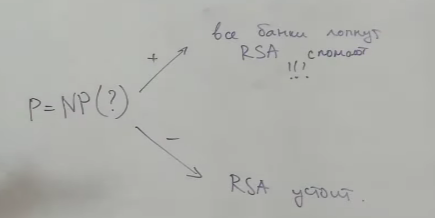
\includegraphics[scale=0.6]{img/kripke_model_greate_ferma_theorem}

\begin{definition}[Модель Крипки]
    Рассмотрим $W_i$ множество миров, имеющие частичный порядок ($\leqslant$).

    Зададим отношение вынужденности $W_i \Vdash P_i$ ($\Vdash \subseteq W_i \times P_i$).

    При этом если $W_j\Vdash P_i$ и $W_j \leqslant W_k$, то $W_k \Vdash P_i$.
\end{definition}

\begin{definition}
Доопределим связки  $\Vdash$ на все выражения:
\begin{enumerate}
    \item $W_i \Vdash \alpha\& \beta$, если $W_i \Vdash \alpha$ и $W_i \Vdash \beta$
    \item $W_i \Vdash \alpha\lor \beta$, если $W_i \Vdash \alpha$ или $W_i \Vdash \beta$
    \item $W_i \Vdash \neg \alpha$, если нет $W_j \geqslant W_i$, что $W_j \Vdash \alpha$
    \item Пусть во всех $W_j \geqslant W_i$ всегда, когда $W_j \Vdash \alpha$, имеет место $W_j \Vdash \beta$, тогда в мире $W_i$ вынуждена импликация $\alpha \to \beta$.
\end{enumerate}
\end{definition}

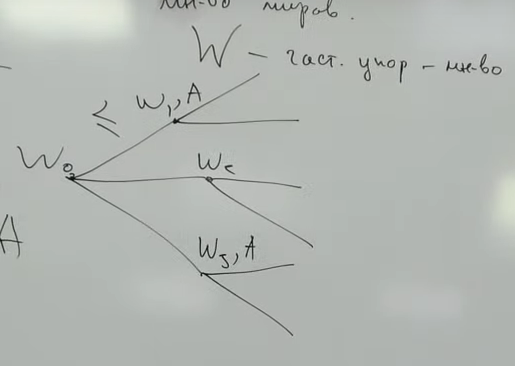
\includegraphics[scale=0.7]{img/forced_variable_worlds}

\begin{definition}
    Если $W_i \Vdash \alpha$ при всех $W_i \in W$, то $\vDash \alpha$ ($\alpha$ общезначима).
\end{definition}


\begin{theorem}
    Модель Крипке~--- корректная модель ИИВ.
\end{theorem}
\begin{proof}
    Пусть $\langle W, \Omega\rangle$~--- топология, $\Omega = \{\tl W \subseteq W \mid$ если  $ W_i\in \tl W, W_i \leqslant W_j$, то $W_j \in \tl W \}$ (множество всех подлесов, где каждый узел присутствует вместе со своим поддеревом).\\
    Пусть $\{W_k \mid W_k \Vdash P_j\}$~--- открытое множество.\\
    Примем $\llbracket P_j \rrbracket = \{ W_k \mid W_k \Vdash P_j\}$, тогда $\llbracket \alpha \rrbracket = \{ W_k \mid W_k \Vdash \alpha\}$.

    Поскольку любая топологическая модель~--- корректная модель ИИВ, то и модель Крипке~--- корректная.
\end{proof}

\begin{definition}
    $\vDash \alpha$ если $W \vdash \alpha$.
\end{definition}

    \begin{theorem}
        У ИИВ нет полной конечной табличной модели.
    \end{theorem}
    \begin{proof}
        $\varphi(n) = \bigvee\limits_{i = 1, j = 1, i \neq j}^{n, n} A_i \to A_{j}$ .

        Пусть $T$~--- модель, $|\mathbb{V}| = n$.

        Рассмотрим $\varphi(n+1)$.  По принципу Дирихле. Есть $A_j$ и $A_i$: $\llbracket A_j \rrbracket = \llbracket A_i \rrbracket$.

        Несложно показать $\llbracket A_i \to A_j\rrbracket = \true \implies$ $\llbracket \varphi(n + 1) \rrbracket = \true$.

        Рассмотрим модель, где $\varphi(n)$ не доказуемо ни при каком $n$.

        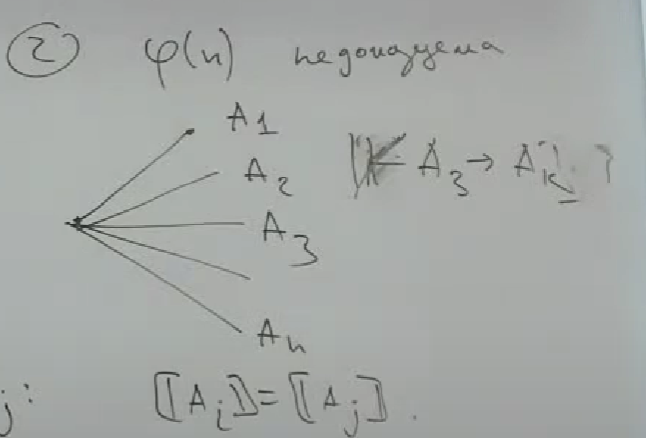
\includegraphics[scale=0.5]{img/iiv_table_model.PNG}

        $\llbracket A_3 \to A_k \rrbracket = \false$.
    \end{proof}

\subsection{Изоморфизм Кари--Ховарда}

\begin{statement}
    $\tau, \sigma$~-- типы.

    $\tau \to \sigma$
    \begin{lstlisting}[mathescape=true]
    f(x : $\tau$): $\sigma$ {
        return g(x);
    }\end{lstlisting}

    $\tau \& \sigma$
    \begin{lstlisting}[mathescape=true]
    f(x: $\tau$, y: $\sigma$)\end{lstlisting}

    $\tau \vee \sigma$
    \begin{lstlisting}[mathescape=true]
    f(x: std:variant<$\tau$, $\sigma$>)\end{lstlisting}

\end{statement}

\begin{definition}
    [Изоморфизм Кари--Ховарда]
    Программа соответствует доказательству.
    Тип соответствует утверждению. ...
    (всё в интуиционистской логике)
\end{definition}

\begin{note}
    $f: \neg\neg \alpha \to \alpha $ -- потом подумаем как это интерпретировать.
\end{note}

\endinput
